\documentclass{standalone}
\usepackage{tikz}
\usetikzlibrary{patterns, positioning}
\usetikzlibrary{shapes.misc}
\usepackage[outline]{contour}
\contourlength{1.5pt} 
\usepackage[sfdefault]{ClearSans} %% option 'sfdefault' activates Clear Sans as the default text font
\usepackage[T1]{fontenc}

\begin{document}
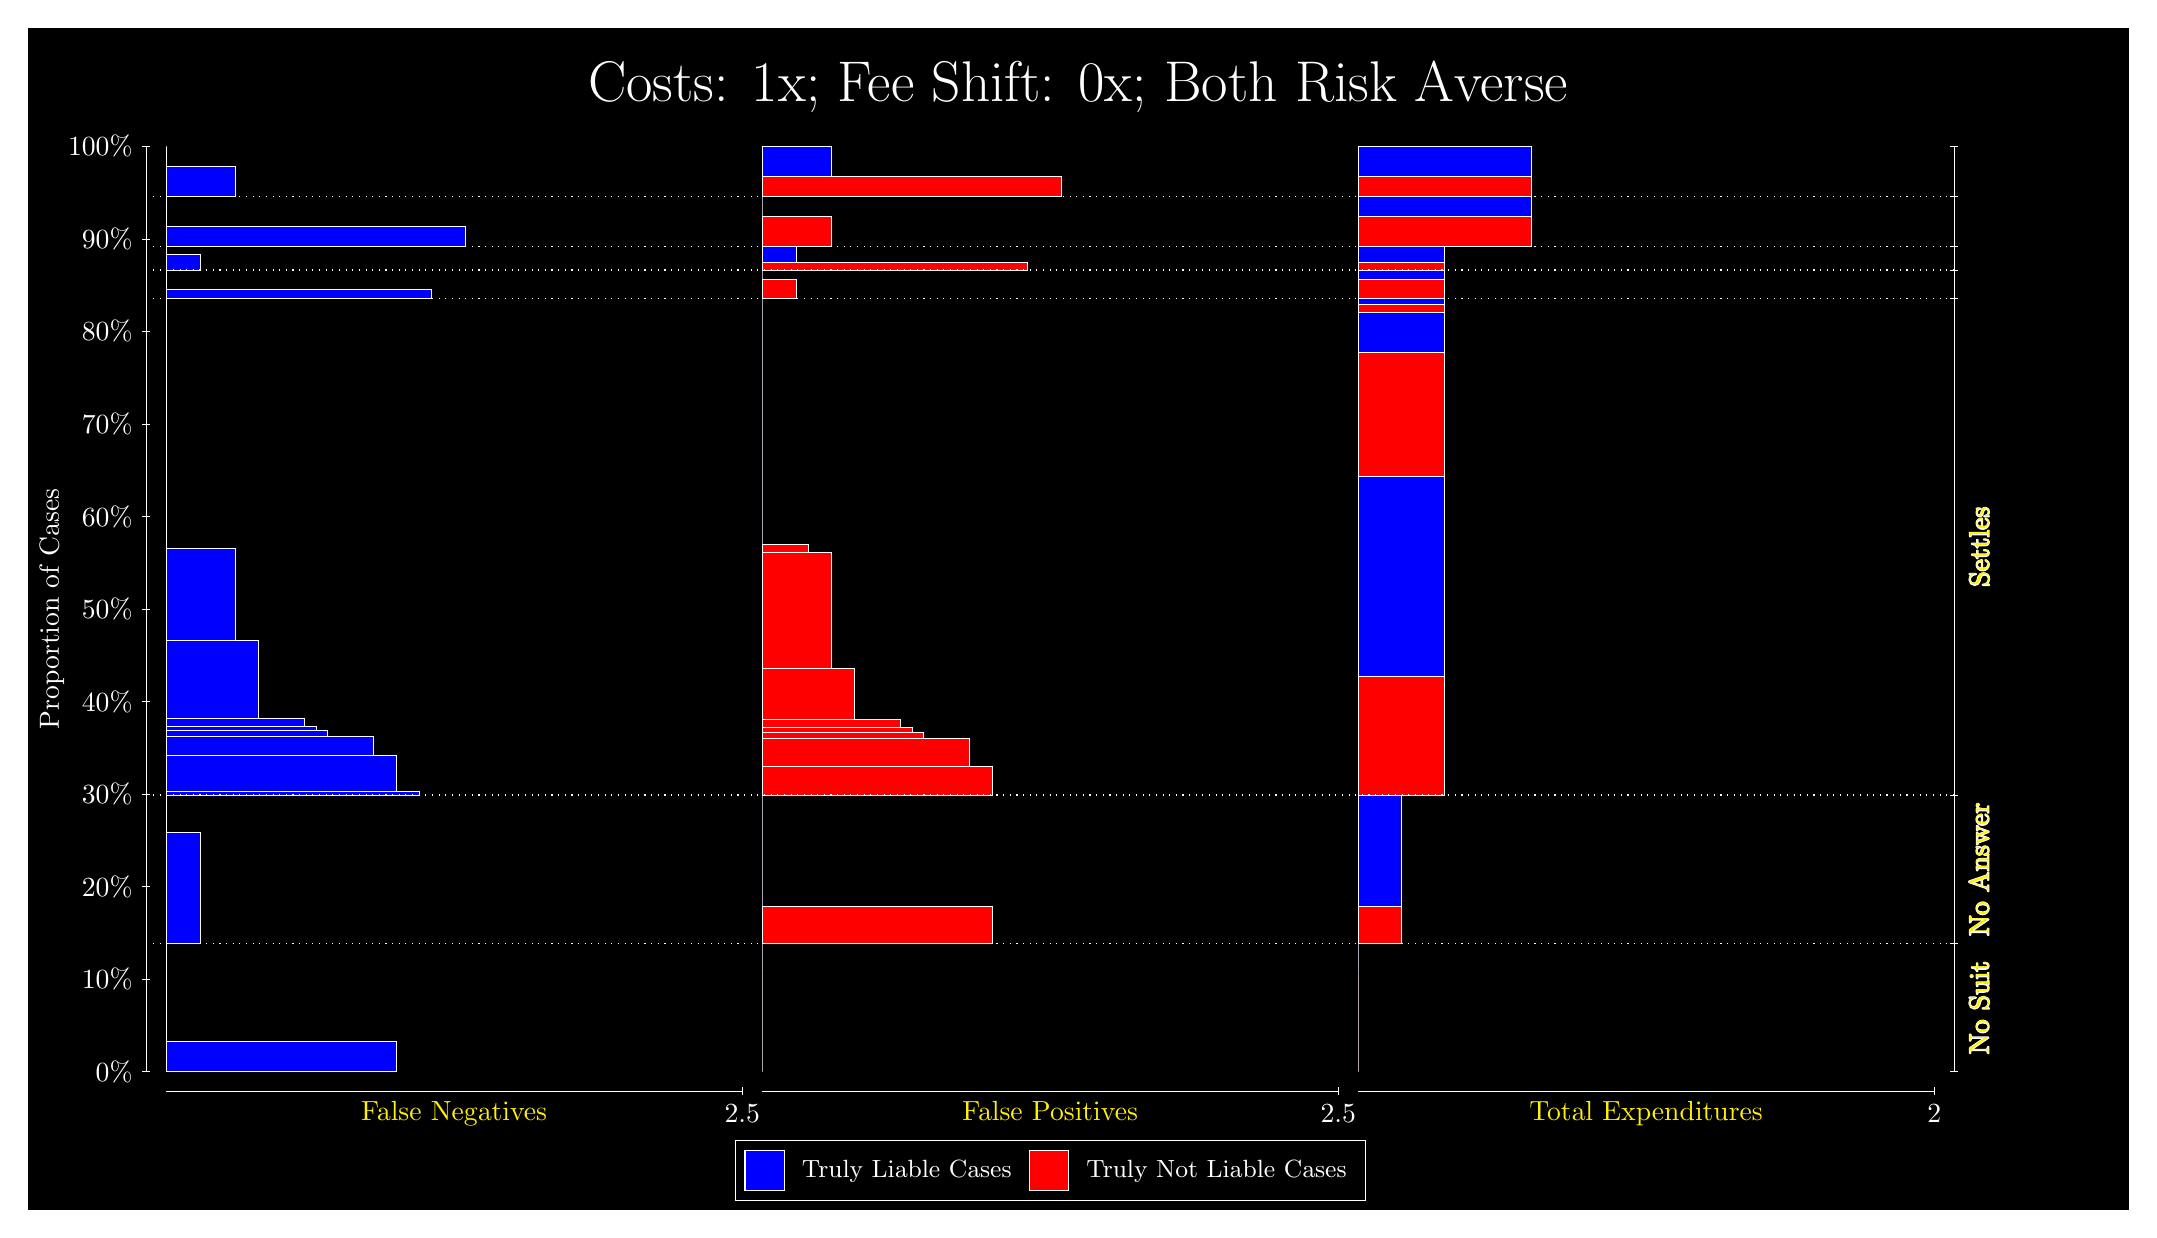
\begin{tikzpicture}
\draw[fill=black] (0,0) rectangle (26.667,15);
\draw[text=white] (0,13.5) rectangle (26.667,15) node[midway] {\huge Costs: 1x; Fee Shift: 0x; Both Risk Averse};
\draw[white, very thin] (1.5,1.75) -- (1.5,13.5);
\node[rotate=90, text=white, anchor=center] at (0.3, 7.625) {Proportion of Cases};
\draw[white, very thin] (1.45,1.75) -- (1.55,1.75);
\node[text=white, anchor=east] at (1.45, 1.75) {0\%};
\draw[white, very thin] (1.45,2.925) -- (1.55,2.925);
\node[text=white, anchor=east] at (1.45, 2.925) {10\%};
\draw[white, very thin] (1.45,4.1) -- (1.55,4.1);
\node[text=white, anchor=east] at (1.45, 4.1) {20\%};
\draw[white, very thin] (1.45,5.275) -- (1.55,5.275);
\node[text=white, anchor=east] at (1.45, 5.275) {30\%};
\draw[white, very thin] (1.45,6.45) -- (1.55,6.45);
\node[text=white, anchor=east] at (1.45, 6.45) {40\%};
\draw[white, very thin] (1.45,7.625) -- (1.55,7.625);
\node[text=white, anchor=east] at (1.45, 7.625) {50\%};
\draw[white, very thin] (1.45,8.8) -- (1.55,8.8);
\node[text=white, anchor=east] at (1.45, 8.8) {60\%};
\draw[white, very thin] (1.45,9.975) -- (1.55,9.975);
\node[text=white, anchor=east] at (1.45, 9.975) {70\%};
\draw[white, very thin] (1.45,11.15) -- (1.55,11.15);
\node[text=white, anchor=east] at (1.45, 11.15) {80\%};
\draw[white, very thin] (1.45,12.325) -- (1.55,12.325);
\node[text=white, anchor=east] at (1.45, 12.325) {90\%};
\draw[white, very thin] (1.45,13.5) -- (1.55,13.5);
\node[text=white, anchor=east] at (1.45, 13.5) {100\%};

\draw[white, very thin] (24.457,1.75) -- (24.457,13.5);
\draw[white, very thin] (24.407,1.75) -- (24.507,1.75);
\node[anchor=west] at (24.407, 1.75) {};
\draw[white, very thin] (24.407,3.3725) -- (24.507,3.3725);
\node[anchor=west] at (24.407, 3.3725) {};
\draw[white, very thin] (24.407,5.2625) -- (24.507,5.2625);
\node[anchor=west] at (24.407, 5.2625) {};
\draw[white, very thin] (24.407,11.568) -- (24.507,11.568);
\node[anchor=west] at (24.407, 11.568) {};
\draw[white, very thin] (24.407,11.929) -- (24.507,11.929);
\node[anchor=west] at (24.407, 11.929) {};
\draw[white, very thin] (24.407,12.231) -- (24.507,12.231);
\node[anchor=west] at (24.407, 12.231) {};
\draw[white, very thin] (24.407,12.867) -- (24.507,12.867);
\node[anchor=west] at (24.407, 12.867) {};
\draw[white, very thin] (24.407,13.5) -- (24.507,13.5);
\node[anchor=west] at (24.407, 13.5) {};

\draw[white, very thin, fill=blue] (1.75,1.75) rectangle (4.6775,2.1292);
\draw[white, very thin, fill=red] (1.75,2.1292) rectangle (1.75,3.3725);
\draw[white, very thin, fill=blue] (1.75,3.3725) rectangle (2.1891,4.7894);
\draw[white, very thin, fill=red] (1.75,4.7894) rectangle (1.75,5.2625);
\draw[white, very thin, fill=blue] (1.75,5.2625) rectangle (4.9703,5.3048);
\draw[white, very thin, fill=blue] (1.75,5.3048) rectangle (4.6775,5.7695);
\draw[white, very thin, fill=blue] (1.75,5.7695) rectangle (4.3848,6.0021);
\draw[white, very thin, fill=blue] (1.75,6.0021) rectangle (3.7993,6.0811);
\draw[white, very thin, fill=blue] (1.75,6.0811) rectangle (3.6529,6.1392);
\draw[white, very thin, fill=blue] (1.75,6.1392) rectangle (3.5065,6.2367);
\draw[white, very thin, fill=blue] (1.75,6.2367) rectangle (2.921,7.2271);
\draw[white, very thin, fill=blue] (1.75,7.2271) rectangle (2.6283,8.3903);
\draw[white, very thin, fill=red] (1.75,8.3903) rectangle (1.75,11.568);
\draw[white, very thin, fill=blue] (1.75,11.568) rectangle (5.1167,11.684);
\draw[white, very thin, fill=red] (1.75,11.684) rectangle (1.75,11.929);
\draw[white, very thin, fill=blue] (1.75,11.929) rectangle (2.1891,12.131);
\draw[white, very thin, fill=red] (1.75,12.131) rectangle (1.75,12.231);
\draw[white, very thin, fill=blue] (1.75,12.231) rectangle (5.5558,12.484);
\draw[white, very thin, fill=red] (1.75,12.484) rectangle (1.75,12.867);
\draw[white, very thin, fill=blue] (1.75,12.867) rectangle (2.6283,13.247);
\draw[white, very thin, fill=red] (1.75,13.247) rectangle (1.75,13.5);
\draw[white, very thin, fill=red] (9.3189,1.75) rectangle (9.3189,2.9933);
\draw[white, very thin, fill=blue] (9.3189,2.9933) rectangle (9.3189,3.3725);
\draw[white, very thin, fill=red] (9.3189,3.3725) rectangle (12.246,3.8456);
\draw[white, very thin, fill=blue] (9.3189,3.8456) rectangle (9.3189,5.2625);
\draw[white, very thin, fill=red] (9.3189,5.2625) rectangle (12.246,5.6226);
\draw[white, very thin, fill=red] (9.3189,5.6226) rectangle (11.954,5.983);
\draw[white, very thin, fill=red] (9.3189,5.983) rectangle (11.368,6.0621);
\draw[white, very thin, fill=red] (9.3189,6.0621) rectangle (11.222,6.1202);
\draw[white, very thin, fill=red] (9.3189,6.1202) rectangle (11.075,6.2177);
\draw[white, very thin, fill=red] (9.3189,6.2177) rectangle (10.49,6.8698);
\draw[white, very thin, fill=red] (9.3189,6.8698) rectangle (10.197,8.3469);
\draw[white, very thin, fill=red] (9.3189,8.3469) rectangle (9.9044,8.4401);
\draw[white, very thin, fill=blue] (9.3189,8.4401) rectangle (9.3189,11.568);
\draw[white, very thin, fill=red] (9.3189,11.568) rectangle (9.758,11.814);
\draw[white, very thin, fill=blue] (9.3189,11.814) rectangle (9.3189,11.929);
\draw[white, very thin, fill=red] (9.3189,11.929) rectangle (12.686,12.029);
\draw[white, very thin, fill=blue] (9.3189,12.029) rectangle (9.758,12.231);
\draw[white, very thin, fill=red] (9.3189,12.231) rectangle (10.197,12.614);
\draw[white, very thin, fill=blue] (9.3189,12.614) rectangle (9.3189,12.867);
\draw[white, very thin, fill=red] (9.3189,12.867) rectangle (13.125,13.119);
\draw[white, very thin, fill=blue] (9.3189,13.119) rectangle (10.197,13.5);
\draw[white, very thin, fill=red] (16.888,1.75) rectangle (16.888,2.9933);
\draw[white, very thin, fill=blue] (16.888,2.9933) rectangle (16.888,3.3725);
\draw[white, very thin, fill=red] (16.888,3.3725) rectangle (17.437,3.8456);
\draw[white, very thin, fill=blue] (16.888,3.8456) rectangle (17.437,5.2625);
\draw[white, very thin, fill=red] (16.888,5.2625) rectangle (17.986,6.7724);
\draw[white, very thin, fill=blue] (16.888,6.7724) rectangle (17.986,9.3141);
\draw[white, very thin, fill=red] (16.888,9.3141) rectangle (17.986,10.884);
\draw[white, very thin, fill=blue] (16.888,10.884) rectangle (17.986,11.391);
\draw[white, very thin, fill=red] (16.888,11.391) rectangle (17.986,11.489);
\draw[white, very thin, fill=blue] (16.888,11.489) rectangle (17.986,11.568);
\draw[white, very thin, fill=red] (16.888,11.568) rectangle (17.986,11.814);
\draw[white, very thin, fill=blue] (16.888,11.814) rectangle (17.986,11.929);
\draw[white, very thin, fill=red] (16.888,11.929) rectangle (17.986,12.029);
\draw[white, very thin, fill=blue] (16.888,12.029) rectangle (17.986,12.231);
\draw[white, very thin, fill=red] (16.888,12.231) rectangle (19.083,12.614);
\draw[white, very thin, fill=blue] (16.888,12.614) rectangle (19.083,12.867);
\draw[white, very thin, fill=red] (16.888,12.867) rectangle (19.083,13.119);
\draw[white, very thin, fill=blue] (16.888,13.119) rectangle (19.083,13.5);
\draw[white, dotted] (1.5,3.3725) -- (24.457,3.3725);
\draw[white, dotted] (1.5,5.2625) -- (24.457,5.2625);
\draw[white, dotted] (1.5,11.568) -- (24.457,11.568);
\draw[white, dotted] (1.5,11.929) -- (24.457,11.929);
\draw[white, dotted] (1.5,12.231) -- (24.457,12.231);
\draw[white, dotted] (1.5,12.867) -- (24.457,12.867);
\draw[white, very thin] (1.75,1.5) -- (9.0689,1.5);
\node[text=yellow, anchor=north] at (5.4094, 1.5) {False Negatives};
\draw[white, very thin] (9.0689,1.45) -- (9.0689,1.55);
\node[text=white, anchor=north] at (9.0689, 1.45) {2.5};

\draw[white, very thin] (9.3189,1.5) -- (16.638,1.5);
\node[text=yellow, anchor=north] at (12.978, 1.5) {False Positives};
\draw[white, very thin] (16.638,1.45) -- (16.638,1.55);
\node[text=white, anchor=north] at (16.638, 1.45) {2.5};

\draw[white, very thin] (16.888,1.5) -- (24.207,1.5);
\node[text=yellow, anchor=north] at (20.547, 1.5) {Total Expenditures};
\draw[white, very thin] (24.207,1.45) -- (24.207,1.55);
\node[text=white, anchor=north] at (24.207, 1.45) {2};

\node[text=yellow, centered, rotate=90] at (24.777, 2.5612) {\contour{white}{No Suit}};
\node[text=yellow, centered, rotate=90] at (24.777, 4.3175) {\contour{white}{No Answer}};
\node[text=yellow, centered, rotate=90] at (24.777, 8.4152) {\contour{white}{Settles}};





\draw (12.978300999999998,1.5) node[draw=none] (baseCoordinate) {};
\begin{scope}[align=center]
        \matrix[scale=0.5, draw=white, below=0.5cm of baseCoordinate, nodes={draw}, column sep=0.1cm]{
            \node[rectangle, draw, minimum width=0.5cm, minimum height=0.5cm, fill=blue] {}; &
            \node[draw=none, font=\small, text=white] (B) {Truly Liable Cases}; &
            \node[rectangle, draw, minimum width=0.5cm, minimum height=0.5cm, fill=red] {}; &
            \node[draw=none, font=\small, text=white] (B) {Truly Not Liable Cases}; \\
            };
\end{scope}

\end{tikzpicture}
\end{document}